\documentclass[a4paper,12pt]{article}

% ---------------------------
% Pacchetti di base
% ---------------------------
\usepackage[utf8]{inputenc}
\usepackage[T1]{fontenc}
\usepackage[italian]{babel}
\usepackage{geometry}
\geometry{margin=2cm}

% ---------------------------
% Grafica e matematica
% ---------------------------
\usepackage{graphicx}
\usepackage{amsmath, amssymb}
\usepackage{float} % Per il posizionamento preciso delle figure

% ---------------------------
% Riferimenti e link
% ---------------------------
\usepackage{hyperref}

% ---------------------------
% Header e footer
% ---------------------------
\usepackage{fancyhdr}
\fancyhf{}
\rhead{Relazione Alessandro Bertolazzi}
\cfoot{\thepage}
\pagestyle{fancy}
\setlength{\headheight}{14.5pt}

% ---------------------------
% Caption senza "Figura X:"
% ---------------------------
\usepackage[labelformat=empty]{caption}

% ---------------------------
% Listings e codice JSON e C++
% ---------------------------
% ---------------------------
% Listings e codice
% ---------------------------
\usepackage{bera}
\usepackage{listings}
\usepackage{xcolor}

% Colori di base
\definecolor{background}{HTML}{EEEEEE}
\definecolor{bluekeywords}{rgb}{0.13,0.13,1}
\definecolor{greencomments}{rgb}{0,0.5,0}
\definecolor{redstrings}{rgb}{0.9,0,0}

% Stile per C++
\lstdefinestyle{cppstyle}{
    basicstyle=\ttfamily\small,
    numbers=left,
    numberstyle=\scriptsize,
    stepnumber=1,
    numbersep=8pt,
    showstringspaces=false,
    breaklines=true,
    frame=lines,
    backgroundcolor=\color{background},
    keywordstyle=\color{bluekeywords}\bfseries,
    commentstyle=\color{greencomments},
    stringstyle=\color{redstrings},
    identifierstyle=\color{black},
    literate=
    {à}{{\`a}}1 {è}{{\`e}}1 {é}{{\'e}}1 {ì}{{\`i}}1 {ò}{{\`o}}1 {ù}{{\`u}}1
}

\lstdefinelanguage{cpp}{
    style=cppstyle,
    keywords={class, public, private, protected, virtual, override, const, auto, return, void, bool, int, double, float, char, string, vector, pair, include, using, namespace, std, constexpr, noexcept, true, false, nullptr},
    morecomment=[l]{//},
    morecomment=[s]{/*}{*/},
    morestring=[b]",
}

% Stile per JSON
\lstdefinestyle{jsonstyle}{
    basicstyle=\ttfamily\small,
    numbers=left,
    numberstyle=\scriptsize,
    stepnumber=1,
    numbersep=8pt,
    showstringspaces=false,
    breaklines=true,
    frame=lines,
    backgroundcolor=\color{background},
    literate=
     *{0}{{{\color{magenta!60!black}0}}}{1}
      {1}{{{\color{magenta!60!black}1}}}{1}
      {2}{{{\color{magenta!60!black}2}}}{1}
      {3}{{{\color{magenta!60!black}3}}}{1}
      {4}{{{\color{magenta!60!black}4}}}{1}
      {5}{{{\color{magenta!60!black}5}}}{1}
      {6}{{{\color{magenta!60!black}6}}}{1}
      {7}{{{\color{magenta!60!black}7}}}{1}
      {8}{{{\color{magenta!60!black}8}}}{1}
      {9}{{{\color{magenta!60!black}9}}}{1}
      {:}{{{\color{red!60!black}{:}}}}{1}
      {,}{{{\color{red!60!black}{,}}}}{1}
      {\{}{{{\color{blue!60!black}{\{}}}}{1}
      {\}}{{{\color{blue!60!black}{\}}}}}{1}
      {[}{{{\color{blue!60!black}{[}}}}{1}
      {]}{{{\color{blue!60!black}{]}}}}{1}
      {"}{{{\color{red!60!black}"}}}{1},
}

% ---------------------------
% Tabelle avanzate
% ---------------------------
\usepackage{tabularx}
\renewcommand{\arraystretch}{1.3} % Più spazio tra righe

% ---------------------------
% Titolo
% ---------------------------
\title{Relazione progetto Programmazione ad Oggetti}
\author{Alessandro Bertolazzi \\ 1227274}
\date{}

\begin{document}

\fontsize{10pt}{12pt}\selectfont
\maketitle

\begin{abstract}
\noindent Relazione del progetto "Biblioteca Virtuale" per il corso "Programmazione ad Oggetti". Un'applicazione scritta in C++ con framework Qt che permette la gestione di una biblioteca. 
\end{abstract}

\section{Introduzione}
Bibliotheca procurator dal latino "direttore della biblioteca", il nome che ho deciso di dare all applicazione. Il progetto proponeva di creare un'applicazione che permettesse la gestione di una biblioteca. L'applicazione che ho deciso di creare non riguarda l'organizzazione di una biblioteca pubblica, bensì l'organizzazione di una biblioteca privata in modo da poter strutturare e catalogare libri, film, CD e simili per un privato con collezioni ampie. Mi sono dedicato questo obbiettivo poiché, oltre a poter avere un'utilità per me, ho notato che non si trovano prodotti simili online e, se si trovano, si tratta di applicazioni datate, a pagamento o non più mantenute.

\section{Struttura del Progetto}
\subsection{Logic}
Nella cartella \texttt{Logic} si trova tutta la parte logica dell'applicazione. Le specifiche del progetto richiedevano almeno 3 classi concrete per i progetti svolti singolarmente, ma per completezza ho deciso di farne 6: \texttt{Anime}, \texttt{SerieTv}, \texttt{Film}, \texttt{Cd}, \texttt{Manga} e \texttt{Libro}. Come classi astratte invece ho utilizzato \texttt{Media} come superclasse e ulteriori due classi \texttt{Series} e \texttt{Cartaceo}.

\begin{figure}[ht!]
    \centering
    
\includegraphics[width=0.6\textwidth]{img/DisegnoSchemaLogico.png}
    \caption{Struttura logica dell'applicazione}
\end{figure}

\subsection{UI}
Per quanto riguarda l'interfaccia grafica, \texttt{mainWindow} gestisce la finestra principale. Ho deciso poi di alleggerire relativamente il file creando file \texttt{Widget} che si occupano di generare parti singole dell'interfaccia. \texttt{topMenuWidget} va a generare la parte di pulsanti che si occupa della creazione, caricamento e chiusura della biblioteca e un bottone per la creazione di nuovi \texttt{Media}. \texttt{rightLayoutWidget} si occupa di gestire la parte destra del layout in cui vengono proposti tutti gli elementi media contenuti nella libreria. \texttt{createItemWidget} invece è la finestra che viene utilizzata a seguito del click del tasto "crea media" per creare un nuovo media. Questa finestra va a sostituire quello che viene inizialmente generato da \texttt{rightLayoutWidget} per poi, una volta confermata la creazione, nascondersi.

\subsection{Service}
Nella parte \texttt{Service} ho cercato di inserire tutta la parte di codice non legata alla generazione della UI e alla logica dell'applicazione. Il file \texttt{jsonService} si occupa della gestione del file JSON per la persistenza dei dati, gestendo il caricamento e il salvataggio del file, conversione e aggiunta di un nuovo media e la rimozione. \texttt{styleUtils} può essere visto come un file CSS nella programmazione web: qui ho raggruppato tutta la parte che si occupa dello stile dell'applicazione (a volte ho lasciato la gestione dello stile direttamente nei file Widget). \texttt{uiService} si occupa invece del "popolamento" dell'interfaccia grafica. \texttt{mediaType} è un file che ho utilizzato per raggruppare i \texttt{dynamic\_cast} presenti nel codice, permettendo una gestione più semplice e pulita dei vari tipi di media. \texttt{mediaService} è la parte che si occupa della gestione generale di tutti i servizi, visto un po' come file "mainService".

\section{Persistenza dei Dati}
Come metodologia di persistenza dei dati ho scelto di utilizzare un file JSON, scelta dettata innanzitutto dalla semplicità di utilizzo e dalla facile manutenibilità. Le modifiche che vengono fatte nell'interfaccia grafica, a seguito della conferma tramite pop-up, vengono scritte subito nel file JSON. La maggior parte del codice di gestione del file JSON è contenuta nel file \texttt{jsonService}.\newline
Il codice JSON è così strutturato:

\begin{lstlisting}[style=jsonstyle]
"media": [
    {
        "anno": 1986,
        "disegnatore": "Akira Toriyama",
        "durataMediaEp": 24,
        "immagine": "../resources/img/dragonball.jpg",
        "inCorso": false,
        "numEpisodi": 153,
        "numStagioni": 5,
        "studioAnimazione": "Toei Animation",
        "titolo": "Dragon Ball",
        "type": "Anime"
    }
]
\end{lstlisting}

\newpage

\section{Interfaccia Grafica}
\begin{figure}[ht!]
    \centering
    \begin{minipage}{0.4\textwidth}
        
\includegraphics[width=\linewidth]{img/TopButton.png}
    \end{minipage}\hfill
    \begin{minipage}{0.55\textwidth}
        \small
        Bottoni del \texttt{topMenuWidget}.\newline
        In ordine:
        \begin{itemize}
            \item Carica una biblioteca esistente
            \item Crea e apre una nuova biblioteca
            \item Chiudi la biblioteca corrente
            \item Crea un nuovo elemento media
        \end{itemize}
        Il secondo bottone, nel caso non sia stata caricata una biblioteca e siano già stati creati dei media, salva automaticamente i media in cache nella nuova biblioteca.
    \end{minipage}
\end{figure}

\begin{figure}[ht!]
    \centering
    \begin{minipage}{0.4\textwidth}
        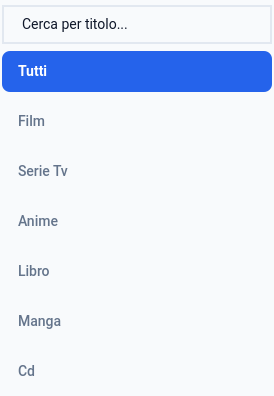
\includegraphics[width=\linewidth]{img/LeftMenu.png}
    \end{minipage}\hfill
    \begin{minipage}{0.55\textwidth}
        \small
        Nel \texttt{leftMenu} viene creata la barra di ricerca che, ad ogni cambiamento (ogni volta che viene digitato un carattere), cerca l'elemento nella biblioteca.\newline
        La ricerca è "case insensitive" e funziona anche con ricerca parziale. Sotto sono presenti i media categorizzati per tipologia.
    \end{minipage}
\end{figure}

\begin{figure}[ht!]
    \centering
    \begin{minipage}{0.4\textwidth}
        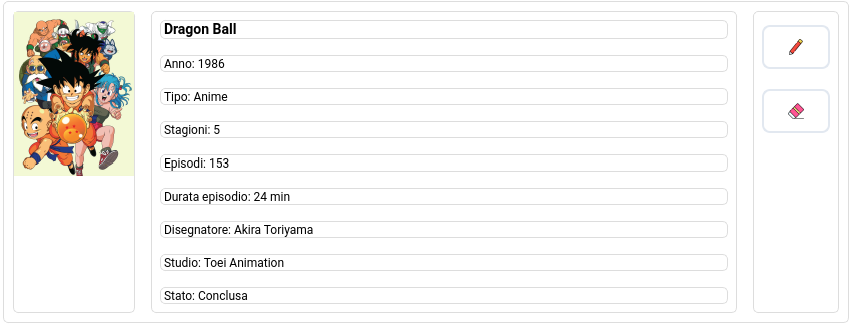
\includegraphics[width=\linewidth]{img/MediaItem.png}
    \end{minipage}\hfill
    \begin{minipage}{0.55\textwidth}
        \small
        Un esempio di elemento media: a sinistra viene caricata l'immagine, mentre a destra vengono visualizzati tutti i dettagli. All'estrema destra ci sono due bottoni: il primo permette di modificare il media, il secondo di cancellarlo dalla libreria. Entrambe le funzioni di modifica ed eliminazione, appena confermate, vanno a modificare direttamente il file JSON.\newline
        Alcuni miglioramenti che non ho implementato: una gestione migliore dello scaling dell'immagine ed un'eventuale ricerca automatica online, per alleggerire l'utente dal dover scaricare e gestire manualmente le immagini.
    \end{minipage}
\end{figure}

\clearpage

\section{Polimorfismo}

\subsection{getSpecificDetails()}

\begin{lstlisting}[language=cpp, style=cppstyle]
\\ Dichiarazione
    virtual std::vector<std::pair<string, string>> getSpecificDetails() const = 0;

\\ Implementazione
    std::vector<std::pair<string, string>> Anime::getSpecificDetails() const {
    auto details = getSeriesBaseDetails(); // Eredita da Series
    details.insert(details.end(), {
        {"Disegnatore", disegnatore},
        {"Studio", studioAnimazione}
    });
    return details;
    }
\end{lstlisting}

La funzione \texttt{getSpecificDetails()} è una funzione virtuale pura definita nella classe astratta \texttt{Media} e ridefinita in ogni classe concreta. Questa funzione viene utilizzata per ottenere i dettagli specifici di ogni tipo di media, restituendo un vettore di coppie chiave-valore che rappresentano gli attributi specifici dell'istanza. Ad esempio, la classe \texttt{Anime} eredita da \texttt{Series} e aggiunge dettagli specifici come "Disegnatore" e "Studio". Ho scelto di utilizzare questo approccio contro all utilizzo di dinamyc\_cast per ottenere i valori specifici di ogni media visto che mantiene il codice piú pulito e leggibile.

\subsection{toJsonSpecific() / fromJsonSpecific()}

\begin{lstlisting}[language=cpp, style=cppstyle]
\\ Dichiarazioni

    virtual QJsonObject toJsonSpecific() const = 0;
    virtual void fromJsonSpecific(const QJsonObject& json) = 0;

\\ implementazione

    QJsonObject SerieTv::toJsonSpecific() const {
    auto json = getSeriesBaseJson();
    json["ideatore"] = QString::fromStdString(ideatore);
    json["casaProduttrice"] = QString::fromStdString(casaProduttrice);
    return json;
    }
\end{lstlisting}

Ho deciso di implementare questo approccio dopo aver provato a gestire i vari tipi di media con dei dynamic\_cast. La gestione dei vari tipi di media con i cast risultava comunque semplice ma rendeva il codice meno leggibile. Con questo approccio poi la serializzazione é "automatica" e non richiede di scrivere i campi specifici per ogni tipo di media. Eventuali modifiche o aggiunte possono essere gestite direttamente nella classe specifica.
\subsection{Clone}

\begin{lstlisting}[language=cpp, style=cppstyle]
\\ Dichiarazione

    virtual Media* clone() const = 0;
\end{lstlisting}

Implementazione del metodo clone senza essere a conoscenza del tipo concreto. Ogni classe specifica gestisce l' allocazione della memoria per il proprio oggetto e garantisce che tutti i dati vengano copiati correttamente.

\subsection{getMediaType()}

\begin{lstlisting}[language=cpp, style=cppstyle]
\\ Dichiarazione

    virtual string getMediaType() const = 0;
\end{lstlisting}

Implementando questa funzione ho potuto rimuovere tutti i dynamic\_cast e typeid. Ho una chiamata diretta permettendomi di non utilizzare cast che in termini di computazione sono costosi e a rischio di errori. Anche qui ogni classe specifica gestisce il proprio tipo.

\section{Rendiconto delle tempistiche}
Quantificare le ore di lavoro richieste dal progetto risulta complicato, in quanto è stato sviluppato trovando il tempo tra lo studio e il lavoro. Escludendo lo studio personale necessario per comprendere il funzionamento di Qt e delle librerie utilizzate, e lo studio più approfondito del linguaggio C++, posso stimare circa 65 ore di sviluppo.

\begin{table}[h!]
\centering
\begin{tabularx}{\textwidth}{p{4cm} p{2cm} p{2cm} X}
\hline
\textbf{Jobs} & \textbf{Scheduled hours} & \textbf{Actual hours} & \textbf{Notes} \\
\hline
Modellazione diagramma UML          & 1  & 2  & Il tempo é stato sforato perché nel corso dello sviluppo del progetto sono state necessarie delle modifiche. \\
Bozza interfaccia Grafica           & 1  & 1  &   \\
Implementazione modello Logico      & 5  & 5  & Implementazione veloce grazie al diagramma UML già deciso. \\
Implementazione Interfaccia grafica & 15 & 20 &   \\
Implementazione parte Service       & 15 & 15 &   \\
Affinamento Progetto                & 5  & 10 & Questo Job sarebbe da includere nella implementazione della parte di Service, ma visto che é stato lavorato anche su altro ho deciso di considerarlo a parte. \\
Debug                               & 5  & 7  & Quantificare il tempo di debug risulta difficile visto che il progetto é stato sviluppato per parti e dopo ogni modifica spesso risultava necessario sistemare qualcosa. Alcuni bug invece sono stati trovati con un uso piú attento dell applicazione. \\
Modifiche Finali                    & 5  & 5  &   \\
\hline
\end{tabularx}
\end{table}

\section{Possibili Miglioramenti}
\begin{itemize}
    \item Implementare una ricerca online della copertina dei media.
    \item Attualmente Serie Tv, Anime e manga sono stati implementati pensando che l' utente sia in possesso di tutti i volumi o episodi di questi. Sarebbe da rendere possibile all'utente di inserire quali volumi o episodi é effettivamente in possesso.
    \item Implementare uno scaling e ridimensionamento delle immagini di copertina migliore.
    \item Implementare tema scuro.
\end{itemize}

\section{Used Words}
\begin{itemize}
    \item Factory Method Pattern: Definizione da \href{https://it.wikipedia.org/wiki/Factory_method}{Wikipedia}  In programmazione, la "factory" o Factory Method Pattern è un design pattern creazionale che permette di creare oggetti senza specificare la classe esatta dell'oggetto da istanziare. Funziona definendo un'interfaccia per la creazione di oggetti, ma lasciando che le sottoclassi decidano quale oggetto specifico creare, delegando così la responsabilità della creazione. Ho utilizzato la parola factory dove ho utilizzato questo desing pattern, essendo una cosa che ho scoperto durante la creazione di questo progetto mi sono fatto aiutare molto da esempi o altri riferimenti online, non sono sicuro dell uso corretto di questo metodo.
    \item Media: viene inteso come qualsiasi elemento singolo che puó essere Cd, Manga, Serie Tv, Libro e Film..
    \item Cast: usata indicando gli static\_cast ma principalmente in questo caso per i dynamic\_cast.
\end{itemize}

\end{document}
